\section{Os espaços $\mathbb R^n$}

Uma forma usual de visualizar o conjunto $\mathbb R$ dos números reais é pensar neste como o conjunto dos pontos de uma reta.
\begin{figure}[ht]
    \centering
    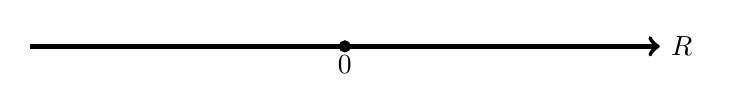
\begin{tikzpicture}
    \draw[->,ultra thick] (-4,0)--(4,0) node[right]{$\mathbb R$};
    \filldraw[black] (0,0) circle (2pt);
    \node[below] at (0,0) {0};

    \end{tikzpicture}
    \caption{A reta real.}
\end{figure}

Lembremos que $\mathbb R^2$ é o conjunto de todos os pares ordenados $(x, y)$, onde $x, y \in \mathbb R$.
Em símbolos:
\begin{equation*}
    \mathbb R^2 = \{(x, y) : x, y \in \mathbb R\}.
\end{equation*}

Em analogia à representação de $\mathbb R$ como uma reta, podemos visualizar $\mathbb R^2$ como o conjunto dos pontos de um plano Cartesiano.
\begin{figure}[ht]
    \centering
    \begin{tikzpicture}
    \draw[->,ultra thick] (-4,0)--(4,0) node[right]{$x$};
    \draw[->,ultra thick] (0,-4)--(0,4) node[above]{$y$};
    % Ponto (2,3)
    \filldraw[black] (2,3) circle (2pt);
    \node[above right] at (2,3) {$(2,3)$};
    \draw[dotted] (2,0) -- (2,3);
    \draw[dotted] (0,3) -- (2,3);
    \draw (2,0.1) -- (2,-0.1);
    \node[below] at (2,0) {2};
    \draw (0.1,3) -- (-0.1,3);
    \node[left] at (0,3) {3};
    \node[below left] at (0,0) {0};

    \end{tikzpicture}
    \caption{O plano Cartesiano.}
\end{figure}

Por sua vez, o conjunto de todas as triplas ordenadas de números reais é denotado por $\mathbb R^3$.
Em símbolos:
\begin{equation*}
    \mathbb R^3 = \{(x, y, z) : x, y, z \in \mathbb R\}.
\end{equation*}

Seguindo o padrão já comentado, podemos visualizar $\mathbb R^3$ como o conjunto dos pontos do espaço tridimensional.

\begin{figure}[ht]
    \centering
    \tdplotsetmaincoords{70}{110}
    \begin{tikzpicture}[tdplot_main_coords]
    % Eixos
    \draw[->,ultra thick] (-4,0,0)--(4,0,0) node[right]{$x$};
    \draw[->,ultra thick] (0,-4,0)--(0,4,0) node[above]{$y$};
    \draw[->,ultra thick] (0,0,-4)--(0,0,4) node[above]{$z$};
    % Ponto (2,3,1)
    \filldraw[black] (2,3,1) circle (2pt);
    \node[above right] at (2,3,1) {$(2,3,1)$};
    % Linhas pontilhadas
    \draw[dotted] (2,0,0) -- (2,3,0) -- (2,3,1);
    \draw[dotted] (0,3,0) -- (2,3,0);
    \draw[dotted] (2,0,0) -- (2,0,1) -- (2,3,1);
    \draw[dotted] (0,0,1) -- (2,0,1);
    % Marcas nos eixos
    \draw (2,0.1,0) -- (2,-0.1,0);
    \node[below] at (2,0,0) {2};
    \draw (0.1,3,0) -- (-0.1,3,0);
    \node[left] at (0,3,0) {3};
    \draw (0.1,0,1) -- (-0.1,0,1);
    \node[left] at (0,0,1) {1};
    \node[below left] at (0,0,0) {0};

    \end{tikzpicture}
    \caption{O espaço tridimensional.}
\end{figure}

No geral, para $n\geq 4$, o conjunto $\mathbb R^n$ é definido como o conjunto de todas as $n$-tuplas ordenadas de números reais:
\begin{equation*}
    \mathbb R^n = \{(x_1, \ldots, x_n) : x_1, \ldots, x_n \in \mathbb R\}.
\end{equation*}

Tal conjunto não possui uma representação gráfica simples a estilo dos anteriores.
Porém, a teoria desenvolvida para $\mathbb R^n$ é uma extensão natural da teoria desenvolvida para $\mathbb R$ e $\mathbb R^2$, e possui amplas aplicações práticas e teóricas.

Elementos de $\mathbb R^n$ serão frequentemente chamados de \emph{pontos} ou \emph{vetores}.
Portanto, para nós, pontos e vetores serão os mesmos objetos matemáticos, e tais palavras podem ser usadas indistintamente.
Porém, a palavra ponto é frequentemente reservada em situações em que pensamos em posições no espaço, enquanto a palavra vetor é mais utilizada em situações em que pensamos na direção, sentido e comprimento determinados pelo ponto com relação a origem $(0, \ldots, 0)$.
\section{Operações em $\mathbb R^n$}

Algumas operações importantes em $\mathbb R^n$ incluem as seguintes.

\begin{definition}
    Sejam $p=(x_1, \ldots, x_n)$ e $q=(y_1, \ldots, y_n)$ dois vetores em $\mathbb R^n$, e $\alpha \in \mathbb R$ um número real.
    A \emph{soma} $p+q$ é definida como:
    \begin{equation*}
        p+q =(x_1, \ldots, x_n)+(y_1, \ldots, y_n)=(x_1+y_1, \ldots, x_n+y_n).
    \end{equation*}
    A \emph{multiplicação por escalar} $\alpha p$ é definida como:
    \begin{equation*}
        \alpha p = \alpha (x_1, \ldots, x_n) = (\alpha x_1, \ldots, \alpha x_n).
    \end{equation*}
    O \emph{produto escalar} $p \cdot q$ é definido como:
    \begin{equation*}
        p \cdot q = (x_1, \ldots, x_n) \cdot (y_1, \ldots, y_n) = x_1y_1 + \ldots + x_ny_n=\sum_{i=1}^n x_iy_i.
    \end{equation*}
    A \emph{norma} de $p$ é definida como:
    \begin{equation*}
        \|p\| = \sqrt{p\cdot p}=\sqrt{x_1^2 + \ldots + x_n^2} = \sqrt{\sum_{i=1}^n x_i^2}.
    \end{equation*}
\end{definition}

Vamos lembrar de importantes interpretações geométricas destas operações.

A soma dos vetores $v=(3, 2)$ e $w=(-1, 1)$ pode ser visualizada como o vetor com início da origem e fim no ponto obtido posicionando-se o vetor $w$ com início no ponto final do vetor $v$, conforme ilustrado abaixo.

\begin{figure}[ht]
    \centering
    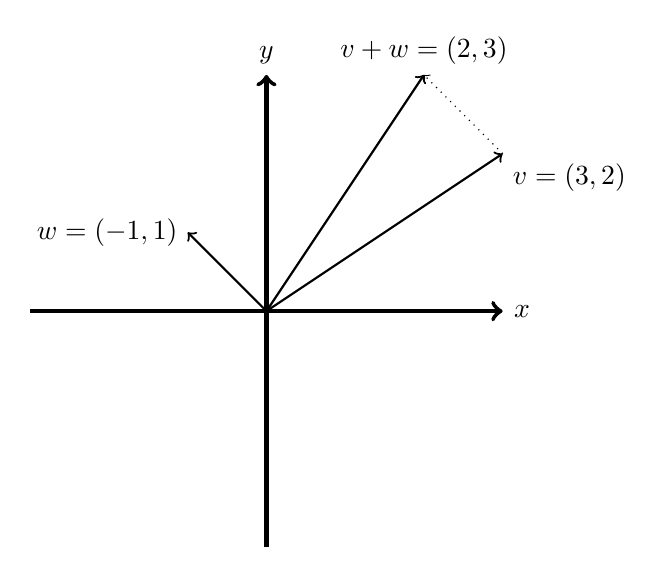
\begin{tikzpicture}
    \draw[->,ultra thick] (-3,0)--(3,0) node[right]{$x$};
    \draw[->,ultra thick] (0,-3)--(0,3) node[above]{$y$};
    % Vetor v=(3,2)
    \draw[->,thick] (0,0) -- (3,2) node[below right]{$v=(3,2)$};
    % Vetor w=(-1,1)
    \draw[->,thick] (0,0) -- (-1,1) node[left]{$w=(-1,1)$};
    % Vetor cópia w=(-1,1)
    \draw[->,dotted] (3,2) -- (2,3);
    % Soma v+w
    \draw[->,thick] (0,0) -- (2,3) node[above, align=left]{$v+w=(2,3)$};
    \end{tikzpicture}
    \caption{Soma de vetores em $\mathbb R^2$.}
\end{figure}
O produto escalar de $v=(1, 2)$ por $2$ e por $-2$ correspondem a, respectivamente, multiplicar o comprimento do vetor $v$ pelo fator $2$, mantendo a direção e sentido, e invertendo o sentido.

\begin{figure}[ht]
    \centering
    \begin{tikzpicture}
    \draw[->,ultra thick] (-3,0)--(3,0) node[right]{$x$};
    \draw[->,ultra thick] (0,-3)--(0,3) node[above]{$y$};

    % Vetor 2v
    \draw[->,thick, draw=blue] (0,0) -- (2,4) node[above right]{$2v=(2,4)$};
    % Vetor 2v
    \draw[->,thick, draw=red] (0,0) -- (-2,-4) node[above right]{$-2v=(-2,-4)$};
    % Vetor v=(1,2)
    \draw[->,thick] (0,0) -- (1,2) node[below right]{$v=(1,2)$};
    \end{tikzpicture}
    \caption{Produto por escalar em $\mathbb R^2$.}
\end{figure}

A norma de um vetor $v=(x_1, \ldots, x_n)$ é o comprimento do vetor que parte da origem até o ponto $(x_1, \ldots, x_n)$ utilizando-se a métrica  usual (Euclidiana) em $\mathbb R^n$.
Vendo $v$ como um ponto no espaço, sua norma denota a distância de $p$ até a origem.

Quanto ao produto escalar, algumas propriedades importantes são as seguintes.

\begin{proposition}
    $p, q, r \in \mathbb R^n$ e $\alpha \in \mathbb R$. Então:
    \begin{enumerate}
        \item $p \cdot q = q \cdot p$ (comutatividade);
        \item $(p+q) \cdot r = p \cdot r + q \cdot r$ (distributividade);
        \item $(\alpha p) \cdot q = \alpha(p \cdot q)$ (associatividade com escalares);
        \item $p \cdot p = \|p\|^2$.
    \end{enumerate}
\end{proposition}

\begin{proof}
    Escrevamos as coordenadas de $p, q, r$ como $p=(x_1, \ldots, x_n)$, $q=(y_1, \ldots, y_n)$ e $r=(z_1, \ldots, z_n)$.

    Para a comutatividade, temos:
    \begin{equation*}
        p \cdot q = \sum_{i=1}^n x_iy_i = \sum_{i=1}^n y_ix_i = q \cdot p.
    \end{equation*}
    Para a distributividade, temos:
    \begin{align*}
        (p+q) \cdot r &= \sum_{i=1}^n (x_i+y_i)z_i \\
        &= \sum_{i=1}^n x_iz_i + \sum_{i=1}^n y_iz_i \\
        &= p \cdot r + q \cdot r.
    \end{align*}
    Para a associatividade com escalares, temos:
    \begin{equation*}
        (\alpha p) \cdot q = \sum_{i=1}^n (\alpha x_i)y_i = \alpha \sum_{i=1}^n x_iy_i = \alpha (p \cdot q).
    \end{equation*}
    Finalmente, temos:
    \begin{equation*}
        p \cdot p = \sum_{i=1}^n x_iy_i = \|p\|^2.
    \end{equation*}
\end{proof}

Algumas propriedades da norma são as seguintes.
\begin{proposition}
    Sejam $v, w \in \mathbb R^n$ e $\alpha \in \mathbb R$. Então:
    \begin{enumerate}[label=(\roman*)]
        \item $\|v\| = 0$ se, e somente se, $v=0$;
        \item $\|\alpha v\| = |\alpha| \|v\|$;
        \item $|v\cdot w| \leq \|v\| \|w\|$ (desigualdade de Cauchy-Schwarz);
        \item $\|v+w\| \leq \|v\| + \|w\|$ (desigualdade triangular).
    \end{enumerate}
\end{proposition}
\begin{proof}
    Vamos verificar cada uma das propriedades. Escreva $v=(x_1, \ldots, x_n)$ e $w=(y_1, \ldots, y_n)$.
    \begin{enumerate}[label=(\roman*)]
        \item Se $v=0$, então $\|v\|=\sqrt{0^2+\ldots+0^2}=0$. Reciprocamente, se $\|v\|=0$, então $\sqrt{\sum_{i=1}^n x_i^2}=0$, o que implica que $x_i=0$ para todo $i$, ou seja, $v=0$.
        \item Temos que $\|\alpha v\| = \sqrt{(\alpha x_1)^2 + \ldots + (\alpha x_n)^2} = |\alpha|\sqrt{x_1^2 + \ldots + x_n^2} = |\alpha| \|v\|$.
        \item Se $w=0$, então a expressão desejada é $0\leq 0$, que é verdadeira.
        Se $w\neq 0$, então, qualquer que seja o número real $t$, temos que:
        \begin{align*}
            0\leq \|v+tw\|^2 &= (v + tw) \cdot (v + tw) \\
            &= v \cdot v + 2t(v \cdot w) + t^2(w \cdot w) \\
            &= \|v\|^2 + 2t(v \cdot w) + t^2\|w\|^2.
        \end{align*}
        Pondo $t=\frac{-v \cdot w}{\|w\|^2}$, temos que:
        \begin{align*}
            0 &\leq \|v\|^2 - 2\frac{(v \cdot w)^2}{\|w\|^2} + \frac{(v \cdot w)^2}{\|w\|^2} \\
            &= \|v\|^2 - \frac{(v \cdot w)^2}{\|w\|^2} \\
            &\iff (v \cdot w)^2 \leq \|v\|^2 \|w\|^2.
        \end{align*}
        Assim, temos que $|v \cdot w| \leq \|v\| \|w\|$.
        \item A desigualdade triangular segue da desigualdade de Cauchy-Schwarz:
        \begin{equation*}
            \|v+w\|^2 = (v+w) \cdot (v+w) = \|v\|^2 + 2v \cdot w + \|w\|^2 \leq \|v\|^2 + 2\|v\|\|w\| + \|w\|^2 = (\|v\| + \|w\|)^2.
        \end{equation*}
    \end{enumerate}
\end{proof}


O produto escalar pode ser utilizado para decidir-se ortogonalidade entre vetores.
É fato conhecido que vale a recíproca do Teorema de Pitágoras: se $\triangle BAC$ é um triângulo, então o ângulo $\angle ABC$ é reto se, e somente se, sendo $a, b, c$ respectivamente as medidas dos segmentos $\overline{BC}, \overline{AC}, \overline{AB}$, temos que $a^2=b^2+c^2$.

\begin{figure}[ht]
    \centering
    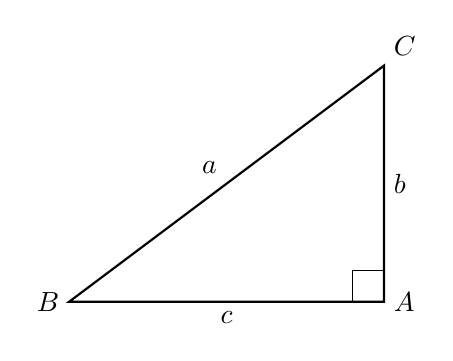
\begin{tikzpicture}
    % Pontos do triângulo
    \coordinate (B) at (0,0);
    \coordinate (A) at (4,0);
    \coordinate (C) at (4,3);

    % Lados do triângulo
    \draw[thick] (B) -- (A) -- (C) -- cycle;

    % Marcação do ângulo reto em B
    \draw (A) ++(-0.4,0) -- ++(0,0.4) -- ++(0.4,0);

    % Nome dos vértices
    \node[right] at (A) {$A$};
    \node[left] at (B) {$B$};
    \node[above right] at (C) {$C$};

    % Lados a, b, c
    \path (B) -- node[above left] {$a$} (C);
    \path (A) -- node[right] {$b$} (C);
    \path (A) -- node[below] {$c$} (B);

    \end{tikzpicture}
    \caption{Triângulo retângulo.}

    No aspecto vetorial, dados dois vetores $v$ e $w$, perceba que o vetor $v+w=v+(-w)$ pode ser representado como o segmento que une as extremidades dos vetores $v$ e $-w$, conforme ilustrado abaixo.

    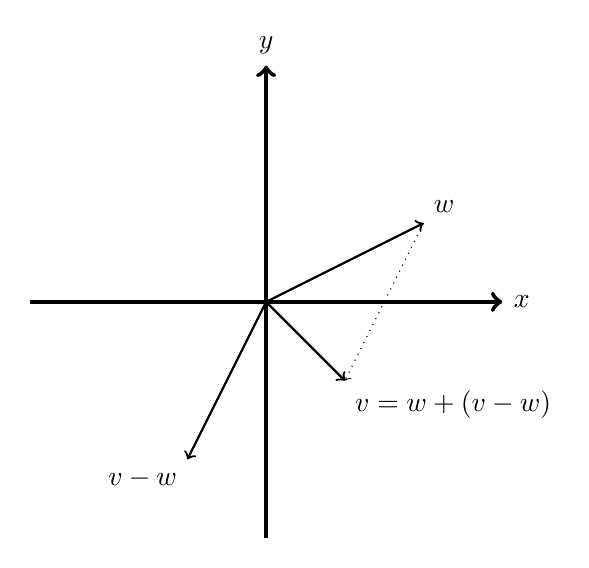
\begin{tikzpicture}
    \draw[->,ultra thick] (-3,0)--(3,0) node[right]{$x$};
    \draw[->,ultra thick] (0,-3)--(0,3) node[above]{$y$};
    % Vetor v
    \draw[->,thick] (0,0) -- (2,1) node[above right]{$w$};
    % Vetor v-w
    \draw[->,thick] (0,0) -- (-1,-2) node[below left]{$v-w$};
    \draw[->,dotted] (2,1) -- (1,-1);
    % Vetor v+w
    \draw[->,thick] (0,0) -- (1,-1) node[below right]{$v=w+(v-w)$};
    \end{tikzpicture}
\end{figure}

Assim, os vetores $v$ e $w$ são ortogonais, se, e somente se, $\|v-w\|^2=\|v\|^2+\|w\|^2$.

\begin{proposition}
    Sejam $v, w \in \mathbb R^n$. Então, $v$ e $w$ são ortogonais se, e somente se, $v \cdot w = 0$.
\end{proposition}
\begin{proof}
    Notemos que, no geral:
    \begin{equation*}
        \|v-w\|^2 = (v-w) \cdot (v-w) = v \cdot v - 2v \cdot w + w \cdot w = \|v\|^2 - 2v \cdot w + \|w\|^2.
    \end{equation*}
    Assim, temos que:
    \begin{align*}
        \|v-w\|^2 &= \|v\|^2 + \|w\|^2 \\
        &\iff \|v\|^2 - 2v \cdot w + \|w\|^2 = \|v\|^2 + \|w\|^2 \\
        &\iff -2v \cdot w = 0 \\
        &\iff v \cdot w = 0.
    \end{align*}
\end{proof}
\section{Distância em $\mathbb R^n$}
A distância entre dois pontos $p, q \in \mathbb R^n$ é dada pela métrica usual (Euclidiana), motivada pelo Teorema de Pitágoras.

\begin{definition}
    Sejam $p, q \in \mathbb R^n$. A \emph{distância (usual, também chamada de Euclidiana)} entre $p$ e $q$ é definida como:
    \begin{equation*}
        d(p, q) = \|p-q\| = \sqrt{(p-q) \cdot (p-q)}=\sqrt{\sum_{i=1}^n (p_i - q_i)^2}.
    \end{equation*}
\end{definition}

Algumas propriedades básicas da distância são as seguintes.
\begin{proposition}
    Sejam $p, q, r \in \mathbb R^n$. Então:
    \begin{enumerate}
        \item $d(p, q) = 0$ se, e somente se, $p=q$.
        \item $d(p, q) = d(q, p)$ (simetria);
        \item $d(p, r) \leq d(p, q) + d(q, r)$ (desigualdade triangular).
    \end{enumerate}
\end{proposition}
\begin{proof}
    Vamos verificar cada uma das propriedades.
    \begin{enumerate}
        \item Dados $p$ e $q$, temos que $d(p, q) = 0$ se, e somente se, $\|p-q\|=0$, o que ocorre se, e somente se, $p-q=0$, ou seja, $p=q$.
        \item Temos que $d(p, q) = \|p-q\| = |-1|\|p-q\| = \|q-p\| = d(q, p)$.
        \item Temos que:
        \begin{align*}
            d(p, r) &= \|p-r\| = \|p-q+q-r\| \\
            &\leq \|p-q\| + \|q-r\| = d(p, q) + d(q, r).
        \end{align*}
    \end{enumerate}
\end{proof}

\section{Bolas e conjuntos abertos em $\mathbb R^n$}
A seguir, definiremos generalizações da noção de intervalo aberto de $\mathbb R$, conceitos essenciais para o futuro estudo de limite, continuidade e diferenciabilidade em $\mathbb R^n$.

\begin{definition}
    Sejam $p \in \mathbb R^n$ e $r>0$. A \emph{bola aberta} de centro $p$ e raio $r$ é o conjunto:
    \begin{equation*}
        B(p, r) = \{q \in \mathbb R^n : d(p, q) < r\}.
    \end{equation*}
    A \emph{bola fechada} de centro $p$ e raio $r$ é o conjunto:
    \begin{equation*}
        \overline B(p, r) = \{q \in \mathbb R^n : d(p, q) \leq r\}.
    \end{equation*}
\end{definition}

Uma bola aberta de raio $r$ centrada em $p$ é ilustrada abaixo.

\begin{figure}[ht]
    \centering
    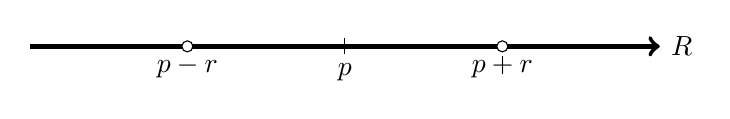
\begin{tikzpicture}
        % Eixo real
        \draw[->,ultra thick] (-4,0)--(4,0) node[right]{$\mathbb R$};
        % Intervalo aberto (p-r, p+r)
        \draw[thick] (-2,0) -- (2,0);
        % Pontos abertos nas extremidades
        \draw[fill=white] (-2,0) circle (2pt) node[below]{$p - r$};
        \draw[fill=white] (2,0) circle (2pt) node[below]{$p + r$};
        % Centro p
        \draw (0,0.1) -- (0,-0.1) node[below]{$p$};
    \end{tikzpicture}
    \caption{Bola aberta de centro $p$ e raio $r$ em $\mathbb R$.}
\end{figure}


\begin{figure}[ht]
    \centering
    \begin{tikzpicture}
    \draw[->,ultra thick] (-4,0)--(4,0) node[right]{$x$};
    \draw[->,ultra thick] (0,-4)--(0,4) node[above]{$y$};
    % Centro da bola
    \filldraw[black] (2,2) circle (2pt);
    \node[below right] at (2,2) {$p$};
    % Raio da bola
    \draw[dashed] (2,2) circle (1.5);
    % Desenho do raio da bola
    \draw[-,thick] (2,2) -- (3.5,2) node[above right]{$r$};
    \end{tikzpicture}
    \caption{Bola aberta de centro $p$ e raio $r$ em $\mathbb R^2$.}
\end{figure}